\documentclass{article}
\usepackage[margin=1in]{geometry}
\usepackage{amsmath}
\usepackage{tikz}
  \usetikzlibrary{calc,decorations.markings,decorations.pathmorphing,arrows.meta}
\begin{document}
%---------------------------------------------------------------------------------
\begin{center}
%
\input{./contour_integral_paths/contour_keyhole.tex}
%
\input{./contour_integral_paths/contour_upper_bc.tex}
%
\input{./contour_integral_paths/contour_dog-bone_center.tex}
%
\input{./contour_integral_paths/contour_dog-bone_right.tex}
%
\input{./contour_integral_paths/contour_upper.tex}
%
\input{./contour_integral_paths/contour_lower.tex}
%
\input{./contour_integral_paths/contour_upper_poles.tex}
%
\input{./contour_integral_paths/contour_2pi_3.tex}
%
\input{./contour_integral_paths/contour_4pi_3.tex}
%
\input{./contour_integral_paths/contour_pi_4.tex}
%
\input{./contour_integral_paths/contour_laplace.tex}
%
\input{./contour_integral_paths/contour_laplace_bc.tex}
%
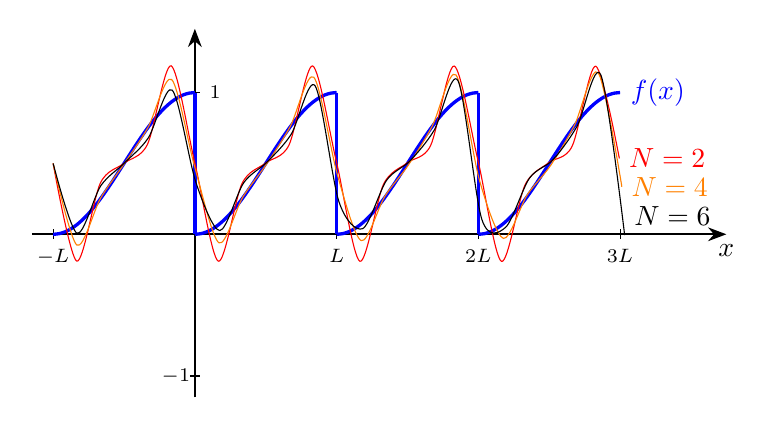
\begin{tikzpicture}[scale=0.9]
  % Configurable parameters
  \def\pie{3.14159265359}
  \newcommand{\axlables}{\normalsize}
  \newcommand{\annotations}{\scriptsize}
  %
  % Axes
  \draw[thick,-Stealth] (-2.3,0) -- (7.5,0)
    node[below] {\axlables$x$};
  \draw[thick,-Stealth] (0,-2.3) -- (0,2.9);
  % Tick labels
  \draw (-2,2pt)  -- (-2,-2pt) node[below] {\annotations$-L$};
  \draw (2,2pt)   -- (2,-2pt)  node[below] {\annotations$L$};
  \draw (4,2pt)   -- (4,-2pt)  node[below] {\annotations$2L$};
  \draw (6,2pt)   -- (6,-2pt)  node[below] {\annotations$3L$};
  \draw (-2pt,-2) -- (2pt,-2)  node[left]  {\annotations$-1$};
  \draw (-2pt,2)  -- (2pt,2)   node[right]  {\annotations$1$};
  %
  % Plots
  \draw[color=blue,smooth,domain=-2:0,very thick] plot (\x,{cos(\x*3.1415/2 r)+1});
  \draw[color=blue,smooth,very thick] (0,2) -- (0,0);
  \draw[color=blue,smooth,domain=0:2,very thick] plot (\x,{-cos(\x*3.1415/2 r)+1});
  \draw[color=blue,smooth,very thick] (2,2) -- (2,0);
  \draw[color=blue,smooth,domain=2:4,very thick] plot (\x,{cos(\x*3.1415/2 r)+1});
  \draw[color=blue,smooth,very thick] (4,2) -- (4,0);
  \draw[color=blue,smooth,domain=4:6,very thick] plot (\x,{-cos(\x*3.1415/2 r)+1}) node[right] {\axlables$f(x)$};
  %
  % N = 2
  \draw[color=red,smooth,domain=-1:6.99]
    plot (\x-1,{3*sin(\x*\pie r)/\pie - 6*sin(2*\x*\pie r)/(3*\pie) +1})
    node[right] {\axlables$N=2$};
  % N = 4
  \draw[color=orange,smooth,domain=-1:7.0255]
    plot (\x-1,{3*sin(\x*\pie r)/\pie - 6*sin(2*\x*\pie r)/(3*\pie) + 3*sin(3*\x*\pie r)/(3*\pie)  - 12*sin(4*\x*\pie r)/(15*\pie) + 1})
    node[right] {\axlables$N=4$};
  % N = 6
  \draw[color=black,smooth,domain=-1:7.065]
    plot (\x-1,{3*sin(\x*\pie r)/\pie - 6*sin(2*\x*\pie r)/(3*\pie) + 3*sin(3*\x*\pie r)/(3*\pie)  - 12*sin(4*\x*\pie r)/(15*\pie) + 3*sin(5*\x*\pie r)/(5*\pie) - 4.5*sin(6*\x*\pie r)/(35*\pie) +1})
    node[above right] {\axlables$N=6$};
\end{tikzpicture}
%
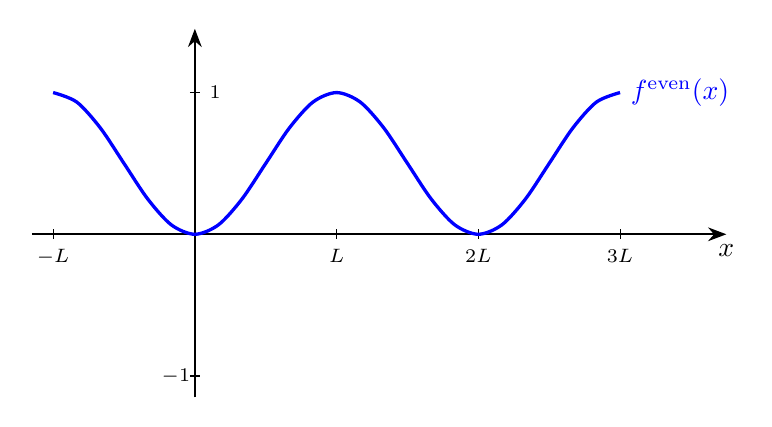
\begin{tikzpicture}[scale=0.9]
  % Configurable parameters
  \def\pie{3.14159265359}
  \newcommand{\axlables}{\normalsize}
  \newcommand{\annotations}{\scriptsize}
  %
  % Axes
  \draw[thick,-Stealth] (-2.3,0) -- (7.5,0)
    node[below] {\axlables$x$};
  \draw[thick,-Stealth] (0,-2.3) -- (0,2.9);
  % Tick labels
  \draw (-2,2pt)  -- (-2,-2pt) node[below] {\annotations$-L$};
  \draw (2,2pt)   -- (2,-2pt)  node[below] {\annotations$L$};
  \draw (4,2pt)   -- (4,-2pt)  node[below] {\annotations$2L$};
  \draw (6,2pt)   -- (6,-2pt)  node[below] {\annotations$3L$};
  \draw (-2pt,-2) -- (2pt,-2)  node[left]  {\annotations$-1$};
  \draw (-2pt,2)  -- (2pt,2)   node[right]  {\annotations$1$};
  %
  % Plots
  \draw[color=blue,smooth,domain=-2:6,very thick] plot (\x,{-cos(\x*\pie/2 r)+1}) node[right] {\axlables$f^{\text{even}}(x)$};
  %\draw[samples=100,color=blue,domain=-2:6,very thick] plot (\x,{2*sin(\x*\pie/4 r)*sin(\x*\pie/4 r)}) node[right] {\axlables$f^{\text{even}}(x)$};
\end{tikzpicture}
%
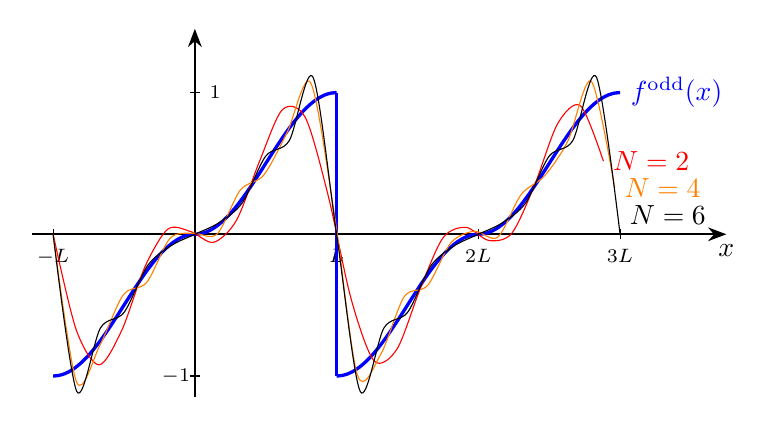
\begin{tikzpicture}[scale=0.9]
  % Configurable parameters
  \def\pie{3.14159265359}
  \newcommand{\axlables}{\normalsize}
  \newcommand{\annotations}{\scriptsize}
  %
  % Axes
  \draw[thick,-Stealth] (-2.3,0) -- (7.5,0)
    node[below] {\axlables$x$};
  \draw[thick,-Stealth] (0,-2.3) -- (0,2.9);
  % Tick labels
  \draw (-2,2pt)  -- (-2,-2pt) node[below] {\annotations$-L$};
  \draw (2,2pt)   -- (2,-2pt)  node[below] {\annotations$L$};
  \draw (4,2pt)   -- (4,-2pt)  node[below] {\annotations$2L$};
  \draw (6,2pt)   -- (6,-2pt)  node[below] {\annotations$3L$};
  \draw (-2pt,-2) -- (2pt,-2)  node[left]  {\annotations$-1$};
  \draw (-2pt,2)  -- (2pt,2)   node[right]  {\annotations$1$};
  %
  % Plots
  \draw[color=blue,smooth,domain=-2:0,very thick] plot (\x,{cos(\x*\pie/2 r)-1});
  \draw[color=blue,smooth,domain=0:2,very thick] plot (\x,{-cos(\x*\pie/2 r)+1});
  \draw[color=blue,smooth,domain=2:4,very thick] plot (\x,{cos(\x*\pie/2 r)-1});
  \draw[color=blue,smooth,domain=4:6,very thick] plot (\x,{-cos(\x*\pie/2 r)+1}) node[right] {\axlables$f^{\text{odd}}(x)$};
  \draw[color=blue,smooth,very thick] (2,2) -- (2,-2);
  %
  % N = 2
  \draw[color=red,smooth,domain=-2:5.765]
    plot (\x,{4*sin(\x*\pie/2 r)/\pie - 8*sin(2*\x*\pie/2 r)/(3*\pie)})
    node[right] {\axlables$N=2$};
  % N = 4
  \draw[color=orange,smooth,domain=-2:5.925]
    plot (\x,{4*sin(\x*\pie/2 r)/\pie - 8*sin(2*\x*\pie/2 r)/(3*\pie) + 4*sin(3*\x*\pie/2 r)/(3*\pie)  - 16*sin(4*\x*\pie/2 r)/(15*\pie)})
    node[right] {\axlables$N=4$};
  % N = 6
  \draw[color=black,smooth,domain=-2:6]
    plot (\x,{4*sin(\x*\pie/2 r)/\pie - 8*sin(2*\x*\pie/2 r)/(3*\pie) + 4*sin(3*\x*\pie/2 r)/(3*\pie)  - 16*sin(4*\x*\pie/2 r)/(15*\pie) + 4*sin(5*\x*\pie/2 r)/(5*\pie) - 6*sin(6*\x*\pie/2 r)/(35*\pie)})
    node[above right] {\axlables$N=6$};
\end{tikzpicture}
\end{center}
%---------------------------------------------------------------------------------
\end{document}